\documentclass[12pt,a4,english,finnish,pdflatex%,handout
]{beamer}
\definecolor{MyGreen}{RGB}{50, 120, 50}
\usecolortheme[named=MyGreen]{structure}

\usepackage{babel}
\usepackage[utf8]{inputenc}
\usepackage[T1]{fontenc}
\usepackage{amsmath,amssymb} 
\usepackage{animate}
\usepackage{multimedia}

\usepackage{natbib}
\bibpunct[: ]{(}{)}{,}{}{}{;}

\usepackage{tikz}

\usepackage{tipa}

\usepackage{hyperref}

\setbeamertemplate{navigation symbols}{}

\graphicspath{{figures/}}

\setlength{\leftmargini}{0pt}
\setlength{\leftmarginii}{1em}

\newcommand{\kommentti}[1]{
  {\bf[#1]}
}

\title{The process of initiating speech and the search for good analysis tools}
\author{Pertti Palo} 
\date{10 Mar 2025} 


\begin{document}

\frame{\titlepage
  \centering
} 

\frame{\frametitle{Outline}
  \begin{itemize}
    \item Introduction
    \item Pixel Difference (PD)
    \item Developments with PD
    \item Spline metrics
    \item Timing
    \item Tools
  \end{itemize}
}


\frame{\frametitle{Introduction}
  \begin{itemize}
  \item In my thesis I concentrated on timing of utterance onset in both
  acoustics and articulation \citep{Palo-MeasuringPrespeechArticulation-2019}.
  \item The data was high-speed tongue ultrasound from a delayed naming
  experiment -- specifically one using the Rastle instructions
  \citep{RastleEtAl-CharacterizingMotorExecution-2005}.
  \end{itemize} 

 	\centering
	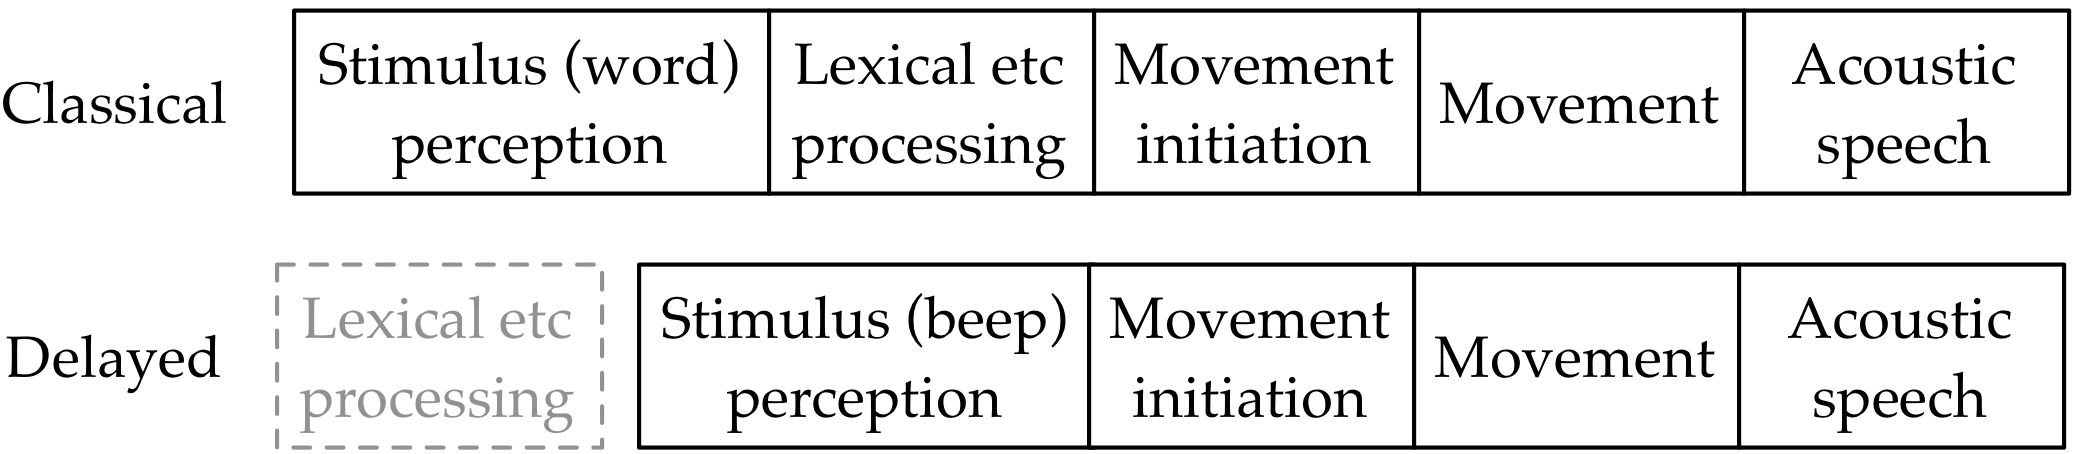
\includegraphics[width=\textwidth]{figures/stages_of_naming.jpg}
}


\frame{\frametitle{Introduction}
  \begin{itemize}
  \item When trying to identify movement onset in greyscale videos with a lot of
  speckle 'noise', it doesn't take long to grow a desire for an easier way.
  \item The speckle 'noise' maybe caused by a number of factors including bubbles in the 
  acoustic gel between the chin and the probe, and more interestingly changes in internal 
  structures of tissues -- such as muscle fibres tensing and relaxing.
  \end{itemize} 
  
  
}


\frame{
  \centering
  {
    \vfill
    \bf \Large 
    \usebeamercolor[fg]{title}
    Pixel Difference (PD)    
    \vfill
%    \includegraphics[height=1.5cm]{figures/aalto_logo} 
  }
}



\frame{\frametitle{Pixel Difference (PD)}
	\begin{itemize}
	\item The first tool out of the box happened to work adequately --  and so for my
	thesis I used Euclidean distance or $l2$-norm to identify articulatory onsets.
	\end{itemize}


	\centering
	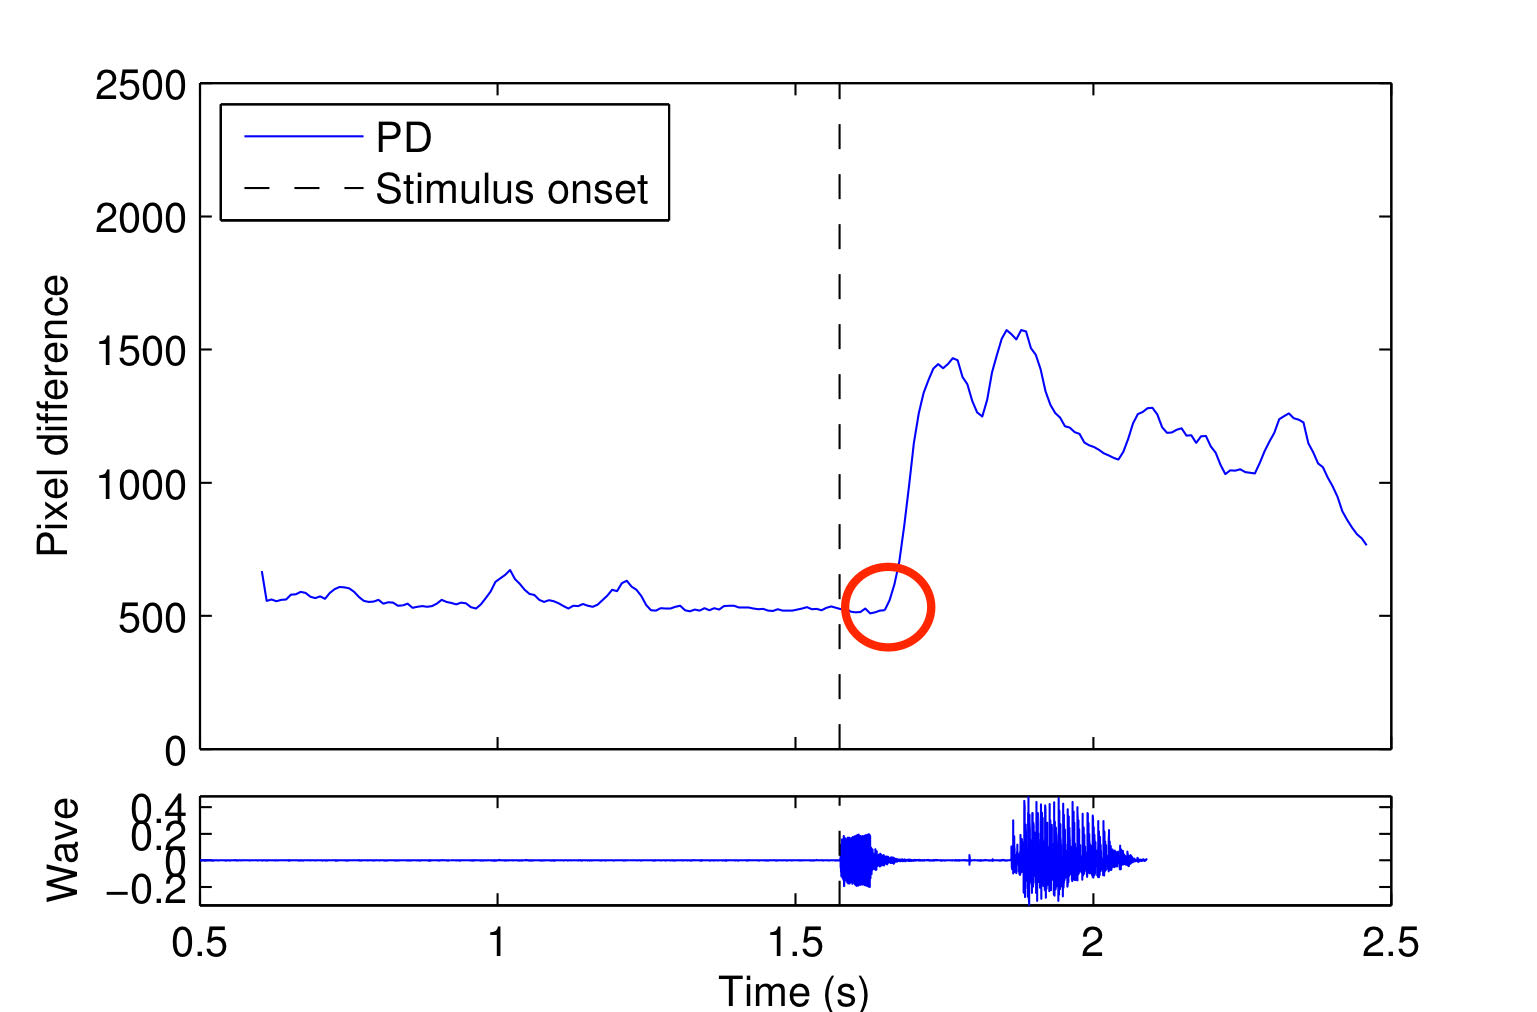
\includegraphics[height=.7\textheight]{figures/pd_caught.jpg}
}

\frame{\frametitle{Pixel Difference (PD): Background}
	\begin{itemize}
		\item The analysis methods presented here are similar to methods
		developed by
		\begin{itemize}
			\item
			 \cite{McMillanCorley-CascadingInfluencesProduction-2010} and
			 \cite{DrakeEtAl-ARTICULATORYEVIDENCEINVOLVEMENT-2013} who used
			 Euclidean distance on ultrasound frames and
			\item \cite{RaeesyEtAl-ParametrisingDegreeArticulator-2011} who
			 used a similar method on MRI data.
		\end{itemize}
		\item The way I have used it, it is actually just the Pythagorean
			theorem applied in a space with a lot more dimensions than~2.
		\end{itemize}
}

\frame{\frametitle{Pixel Difference (PD): Raw vs. Interpolated}
	\begin{itemize}
		\item PD is usually calculated on 
		\begin{itemize}
			\item (a) uninterpolated (probe-return) ultrasound data instead of
			\item (b) interpolated (human-readable) data.
		\end{itemize}
	\end{itemize}
	\centering
	\includegraphics[height=.7\textheight]{figures/raw_and_interpolated.jpg}

	}

\frame{\frametitle{Pixel Difference (PD): The maths}
	\begin{equation*}
	l2(t+0.5) = \sqrt{\sum_{i, j} (x(i,j,t+1) - x(i,j,t))^2}
	\end{equation*}

	\begin{itemize}
		\item $i$ and $j$ are indices that span the width and height of the
		image, $t$ is the time index.
		\item Like said, this is actually just the Pythagorean theorem applied
		in a space with a lot more dimensions than 2.
	\end{itemize}

	}

\frame{\frametitle{Pixel Difference (PD): The maths visually}
	\centering
	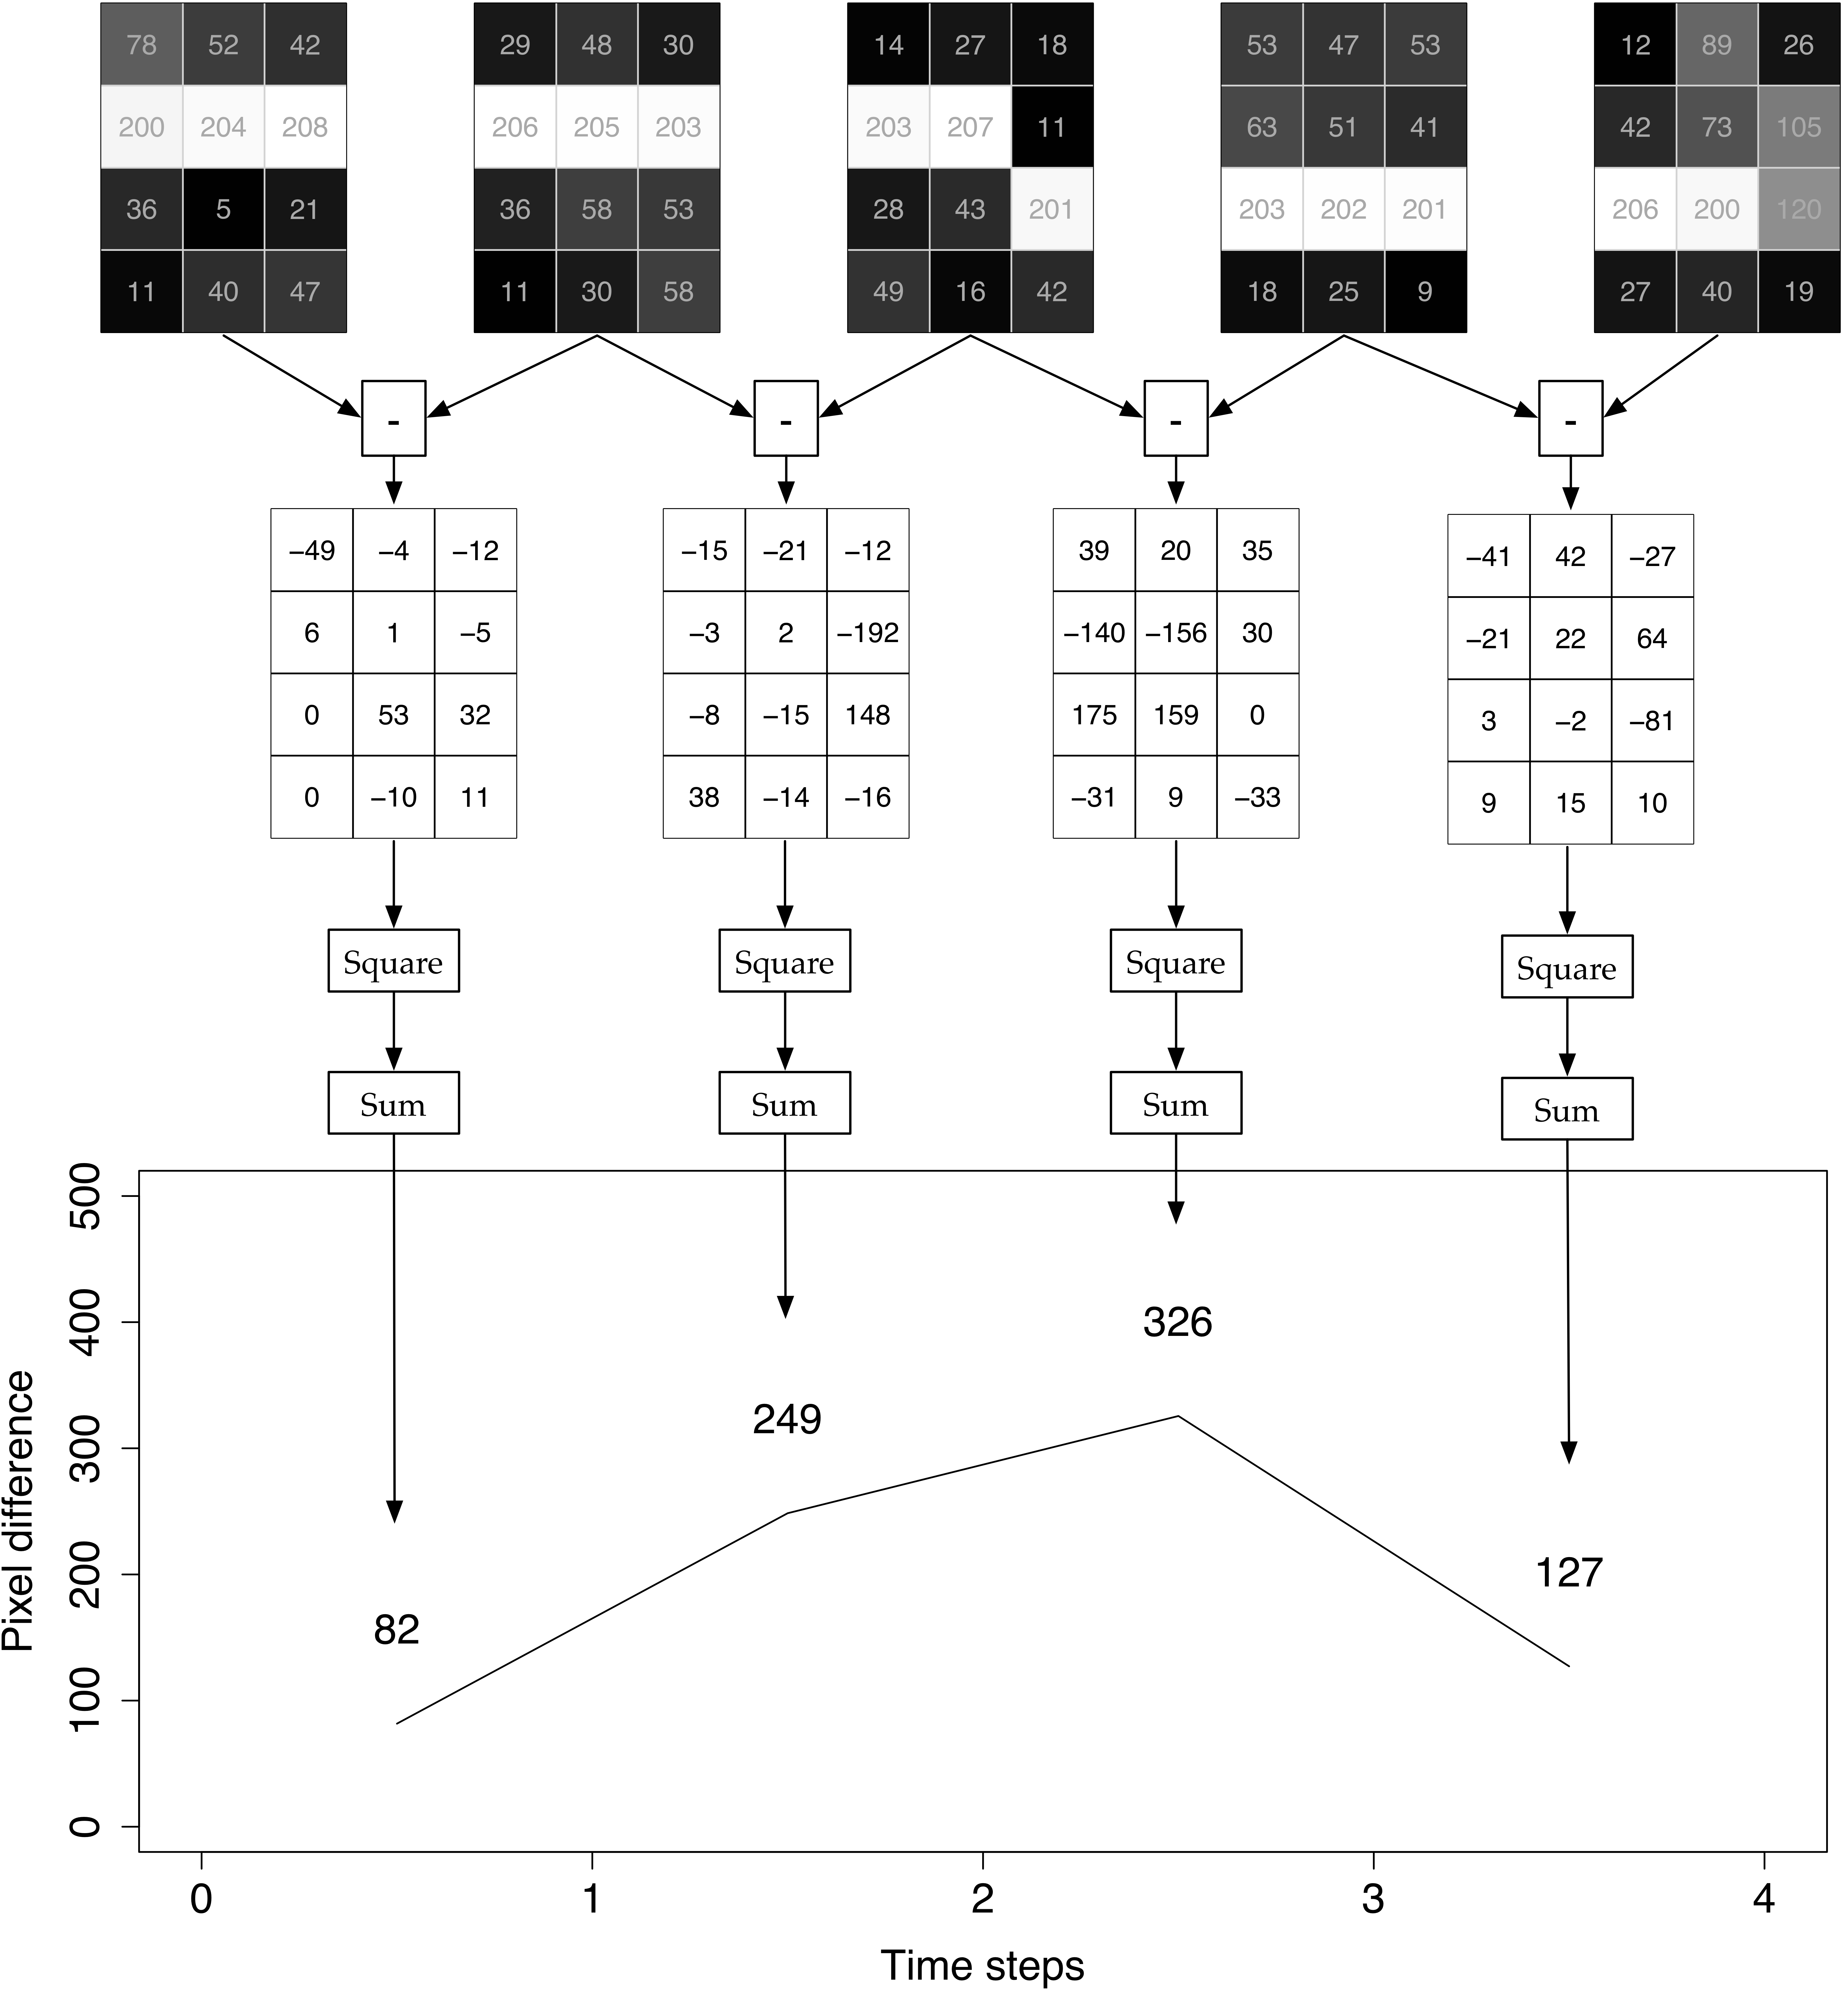
\includegraphics[height=.8\textheight]{figures/pixel_difference_demo_noise_square_sum_tall.png}
}

\frame{
  \centering
  {
    \bf \Large 
    \usebeamercolor[fg]{title}
    \vfill
    Developments with PD
    \vfill
%    \includegraphics[height=1.5cm]{figures/aalto_logo} 
  }
}


\frame{\frametitle{Delayed naming results: Articulatory to Acoustic Interval}
	\begin{center}
		\vspace*{-.5cm}
		\hspace*{-1cm}
		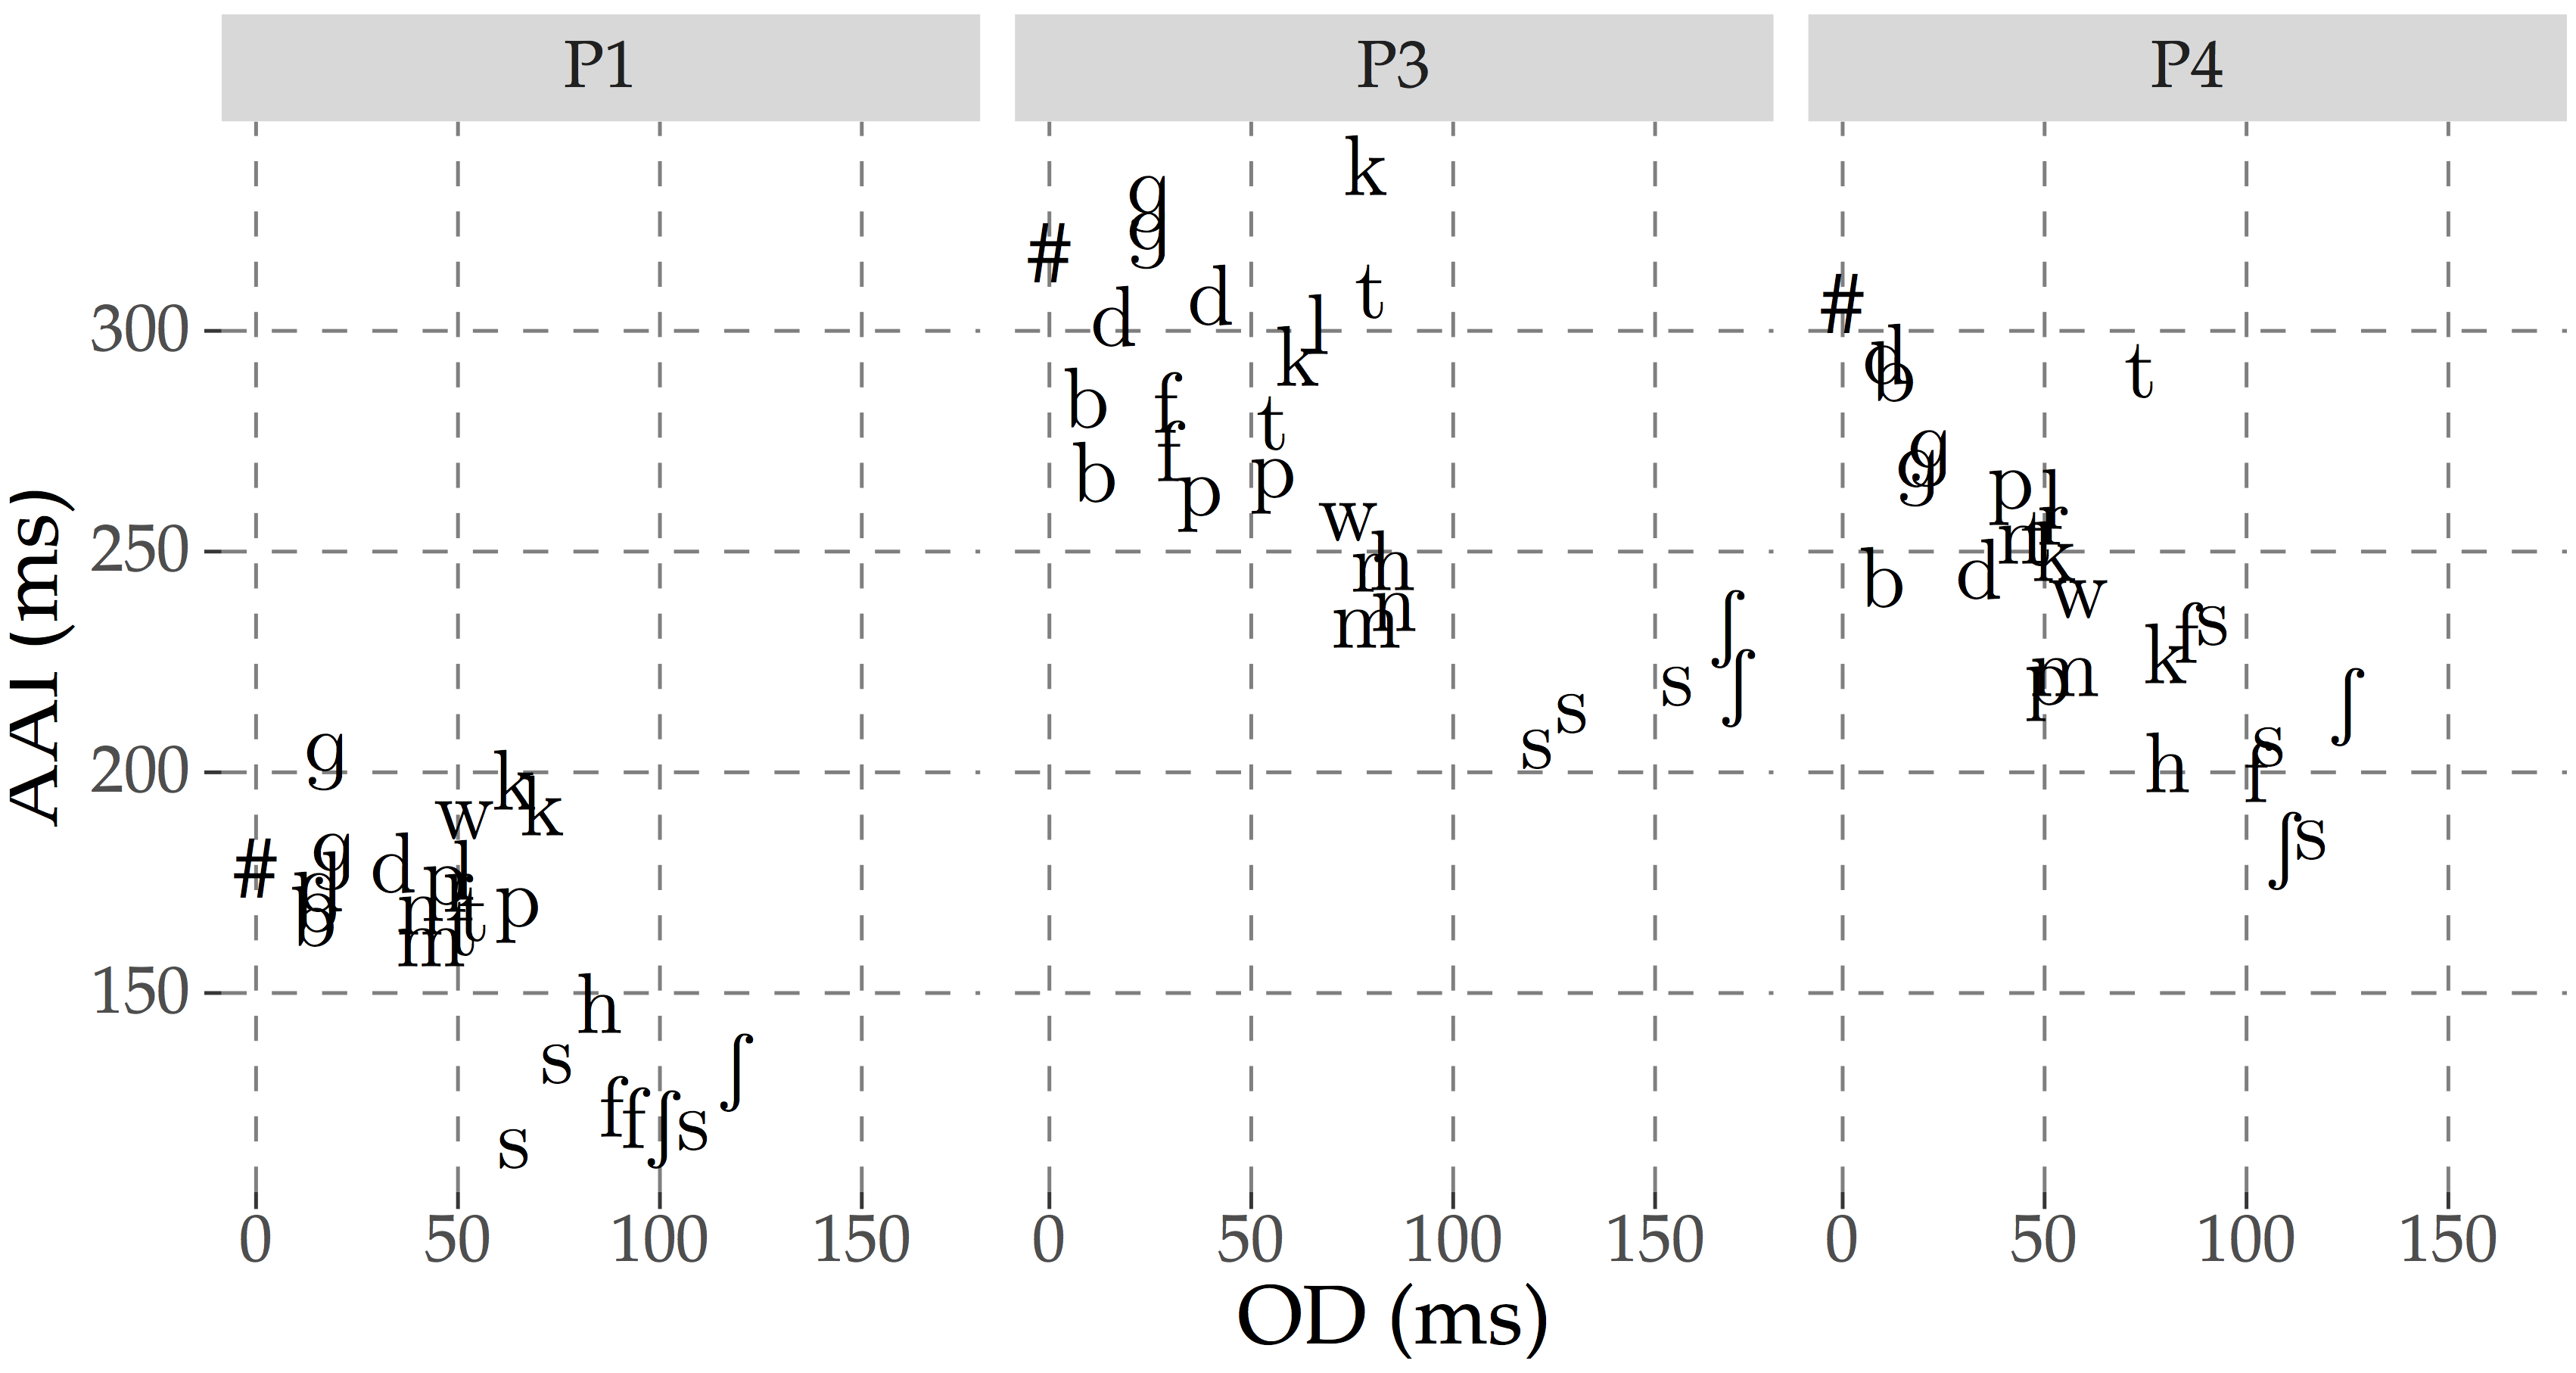
\includegraphics[width=\textwidth]{figures/OD_vs_AAI.jpg}
	\end{center}
	Medianised within participant, over several repetitions and over
	the vowels \textipa{/a,i,O/}. Over all analysable n = 1386: 439 from P1, 672 from P3,
	and 275 from P4.
}

\frame{\frametitle{Theory: Effect of OD on AAI}
	\begin{itemize}
		\item As the Onset Duration (OD) gets longer, Articulatory to Acoustic
		Interval (AAI) shortens.
		\item First three lines represent individual utterances, final line is
		a conceptual model of the effect of continuously lengthening OD.6
	\end{itemize}
	\begin{center}
		\hspace*{-.5cm}
		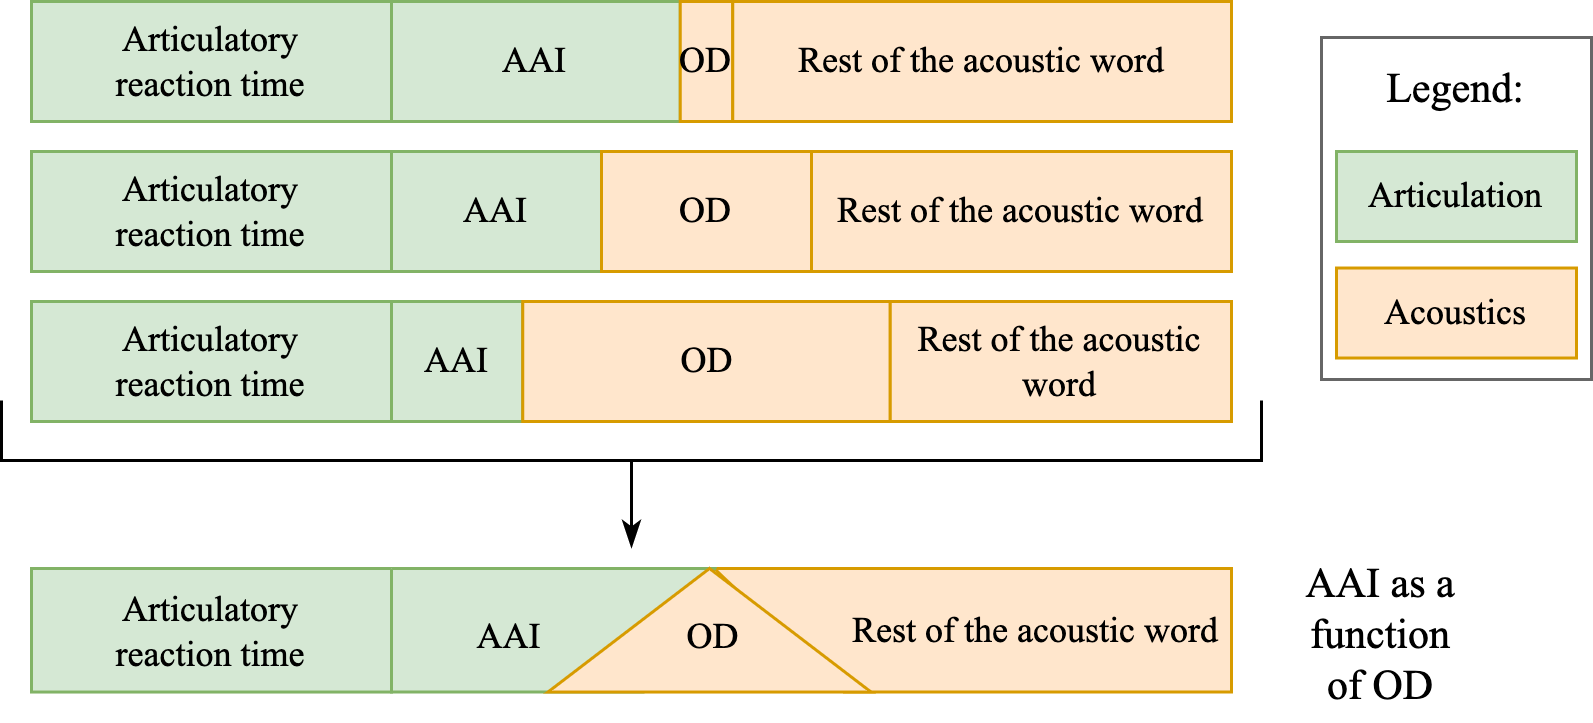
\includegraphics[width=1.1\textwidth]{effect_of_OD.drawio.png}
	\end{center}
}

\frame{\frametitle{Theory: Effect of articulatory rate on AAI}
	\begin{itemize}
		\item If we keep the utterance content constant but vary articulation
		rate, all parts (AAI, OD, and acoustic word) get longer as articulation
		rate goes down.
	\end{itemize}
	\begin{center}
		\hspace*{-.5cm}
		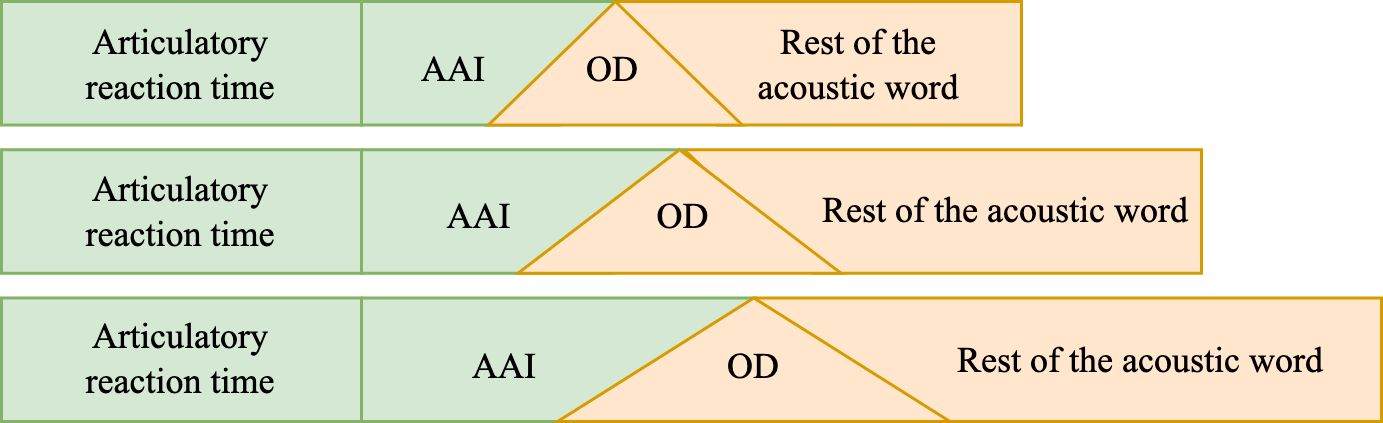
\includegraphics[width=\textwidth]{effect_of_RhymeDur.drawio.png}
	\end{center}
}

\frame{\frametitle{Starting position}
	\begin{itemize}
		\item 'Remain at rest' does not define what 'rest' means.
	\end{itemize}
	\centering
	\hspace*{-.9cm}
	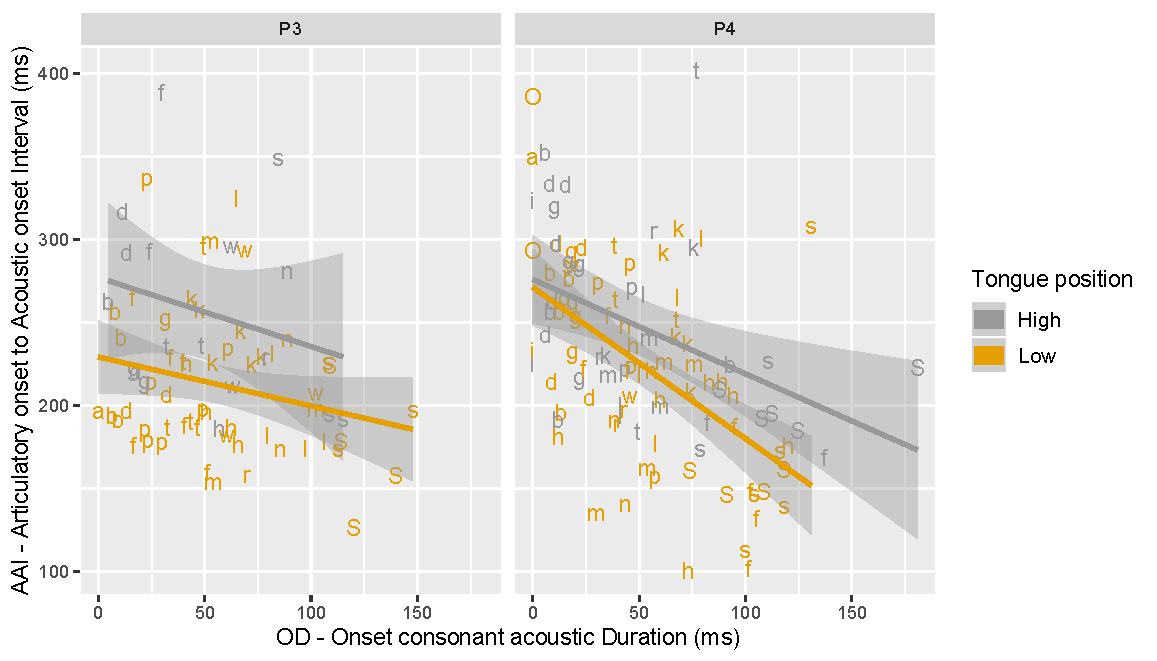
\includegraphics[width=1.17\linewidth]{figures/OD_vs_AAI_smoothsP3P4.pdf}
	% \includegraphics[width=.8\linewidth]{figures/raw_interpolated_2D_step5}
	
}


\frame{\frametitle{References}
  
\bibliographystyle{apalike}
\bibliography{main}

}

\frame{
  \centering
  {
    \bf \Large 
    \usebeamercolor[fg]{title}
    Something else i.e. section title
    
    \vfill
%    \includegraphics[height=1.5cm]{figures/aalto_logo} 
  }
}


\end{document}

